\section{La reconnaissance d'entités nommées~: découverte et enjeux}
N'ayant aucune connaissance préalable sur le traitement du langage naturel, ou NLP pour \textit{Natural Language Processing}, dont la reconnaissance d'entités nommées, ou NER pour \textit{Named Entity Recognition} fait partie, il faut adapter ma démarche. Tout d'abord en se documentant sur le sujet, puis en lisant des publications de recherche, afin de connaître l'état de l'art, et enfin en développant un premier service, pour en avoir une vision pratique. Cette démarche a été grandement facilitée par les moyens techniques mis à ma disposition.
\newline

\subsection{La reconnaissance d'entités nommées pour l'Insee}

\subsubsection{Le traitement du langage naturel}
Le traitement du langage naturel est un domaine qui s'attache, à partir d'un texte, à en analyser le sens et à en extraire une connaissance. Il permet par exemple d'analyser les sentiments dans un texte, ou encore à repérer les mentions d'organisations ou de personnes.
\newline

Il prend la forme d'un «~pipeline~», c'est-à-dire une succession de traitements, chacun donnant une information différente sur le texte. Parmi les traitements les plus courants on trouve~:
\begin{enumerate}
    \item \textit{Tokenisation}~: un pré-traitement qui permet de découper les textes en «~tokens~» à savoir en mots et éléments de ponctuation.
    \vspace{5pt}
    \item \textit{Sentence Split}~: un second pré-traitement qui permet de découper les textes en phrases ou propositions suivant les langues.
    \vspace{5pt}
    \item \textit{Part-of-speech tagging}~: un premier traitement donnant pour chaque token sa nature grammaticale (verbe, adjectif, nom, ponctuation, etc.)
    \vspace{5pt}
    \item \textit{Lemmatisation}~: un traitement souvent complémentaire au précédent, il s'attache à donner, pour chaque mot, l'entrée du dictionnaire de la langue correspondante. Pour un verbe conjugué par exemple, le lemme correspond à l'infinitif.
    \vspace{5pt}
    \item \textit{Dependencies}~: un traitement proposition par proposition, ou phrase par phrase, donnant les dépendances entre les mots. Par exemple quel adjectif est rattaché à quel nom, quel adverbe à quel verbe.
\end{enumerate}
\vspace{10pt}

\begin{figure}[H]
    \centering
    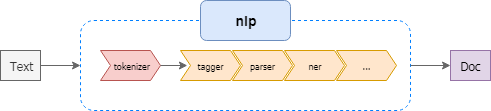
\includegraphics[scale=0.34]{images/Pipeline-example.png}
    \caption{Exemple de pipeline NLP}
    \label{fig:nlp-pipeline-example}
\end{figure}

\vspace{10pt}

On obtient en sortie de ce pipeline des informations à divers niveaux~: \textit{Part-of-speech tagging} et \textit{Lemmatisation} opèrent sur les mots, tandis que \textit{Dependencies} opère sur les phrases et propositions. D'autres traitements, tels que \textit{Coreference resolution} opèrent sur des textes; ce traitement permet de relier les pronoms et autres noms lorsqu'ils font référence à la même entité. Des exemples pour chaque traitement sont donnés en annexe page \pageref{nlp-exemple}.
\newline

Les différentes techniques du traitement du langage naturel, jusqu'alors peu généralisables, ont beaucoup évolué suite à l'arrivée des techniques à base de réseaux de neurones entre 2015 et 2017. C'est pourquoi ce domaine atteint aujourd'hui de meilleures performances, notamment en ce qui concerne la reconnaissance d'entités nommées. Les nouvelles techniques donnent des résultats plus précis, tout en gardant des temps de traitements équivalents aux techniques classiques.
\label{section 2.1.1}

\subsubsection{La reconnaissance d'entités nommées}

\subsubsection*{REN et Désambiguïsation}
La reconnaissance d'entités nommées est l'étiquetage dans un texte d'un mot ou d'un groupe de mots, ainsi que la classification de ce mot ou groupe de mots. Ces classes comprennent de façon générique les personnes, les dates, les lieux ou encore les organisations (instituts, associations, entreprises, etc.). Ce traitement inclut souvent un autre traitement que l'on appelle \textit{Entity Linking} ou \textit{Disambiguation}, qui est le fait de rattacher une occurrence d'entités nommées dans un texte à une base de connaissance, en utilisant le contexte. Prenons un exemple tiré d'\href{https://ambiversenlu.mpi-inf.mpg.de/}{Ambiverse NLU} \cite{ambiverse-nlu}, un service développé par l'Institut de recherche Max Planck effectuant ces deux traitements~:
\newline

\begin{figure}[H]
    \centering
    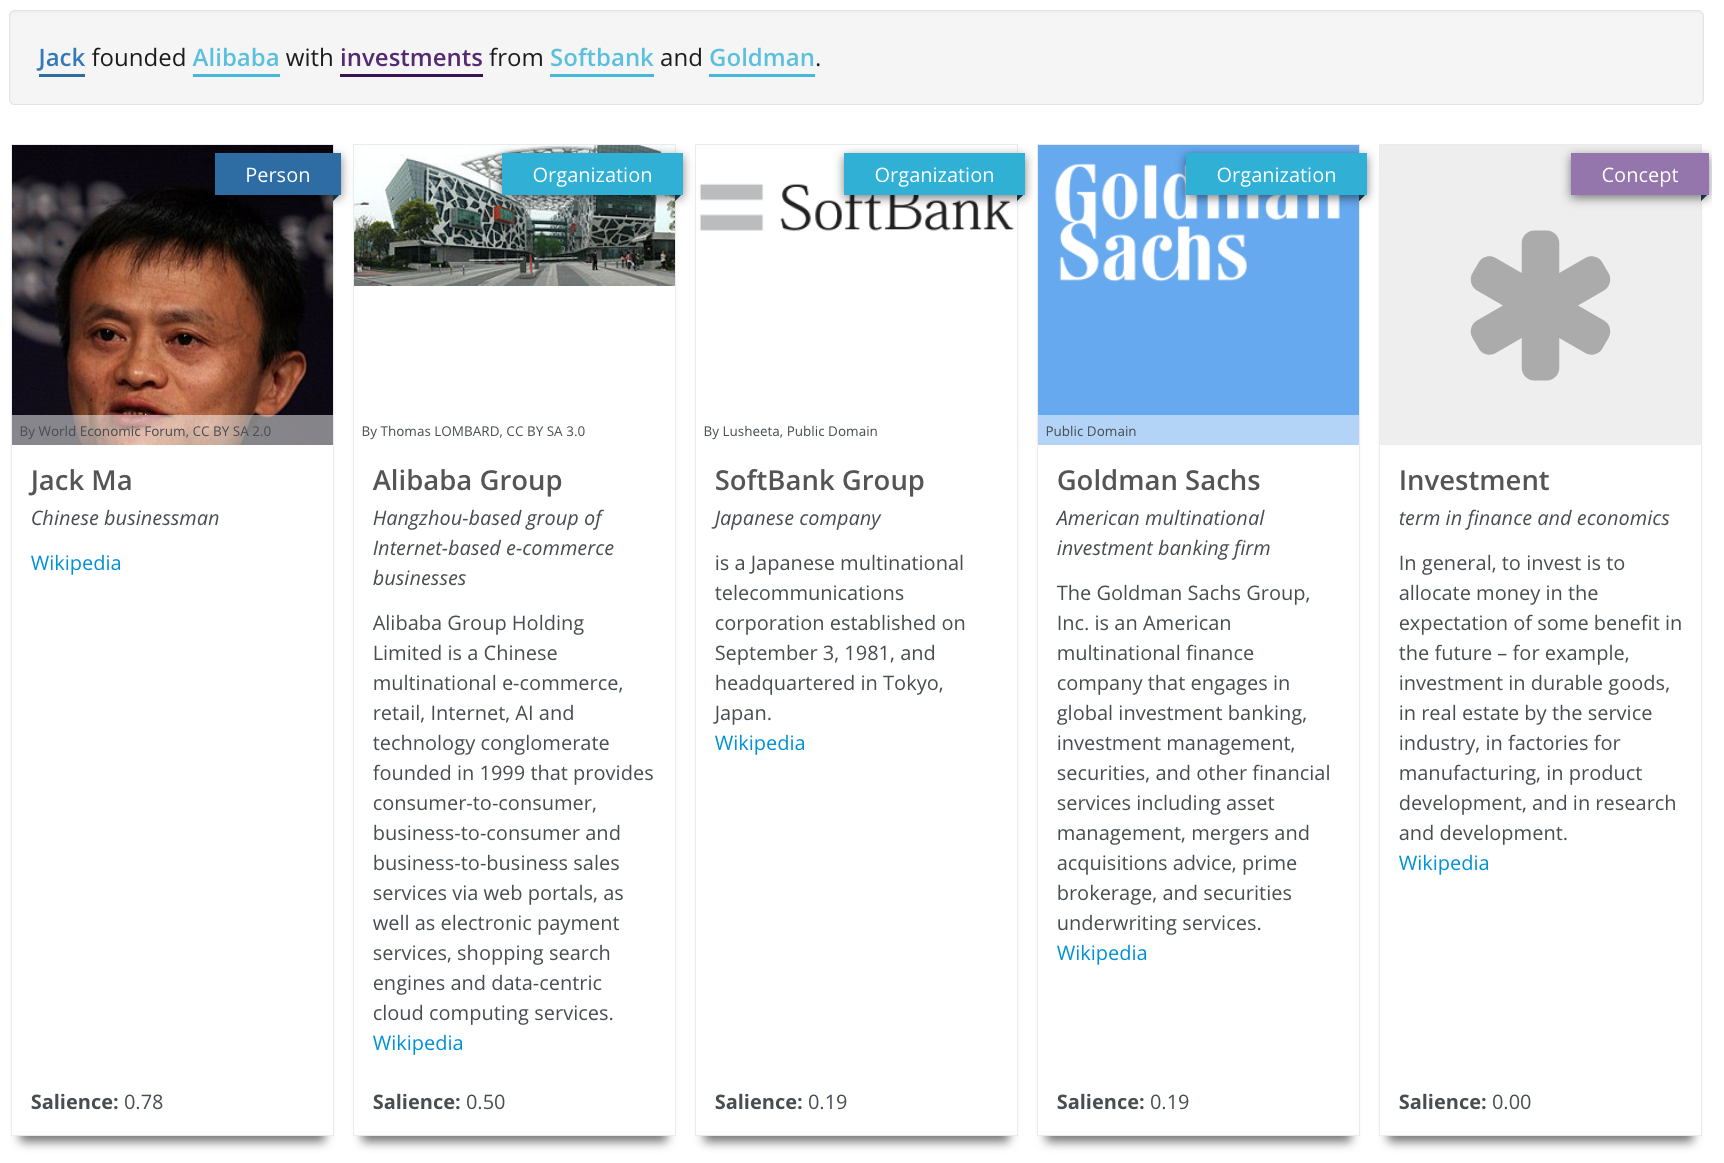
\includegraphics[scale=0.24]{images/ner-demo.png}
    \caption{Exemple de REN et de Désambiguisation}
    \label{fig:ner-demo}
\end{figure}

\vspace{10pt}

Dans la phrase d'exemple çi-dessus, la reconnaissance d'entités nommées à proprement parler est le fait d'étiqueter les quatre premiers caractères, c'est-à-dire le mot «~Jack~», comme faisant mention d'une personne. La désambiguïsation est le fait de lier le mot «~Jack~», dans le contexte de la phrase à Jack Ma. Dans le cas d'Ambiverse NLU, c'est la base donnée DBPedia, graphe RDF généré à partir des données de Wikipedia, qui est utilisée comme base de connaissance.
\newline

Dans la littérature, beaucoup s'interrogent sur la définition d'une entité, plus particulièrement sur les classes utilisées dans la reconnaissance d'entités nommées. Doit-on rester générique, en utilisant la classe «~personne~», laissant un travail de désambiguïsation plus conséquent ? Ou alors doit-on être plus spécifique en utilisant son statut (peintre, musicien, chef d'entreprise) ?

La question se pose également dans le cas des concepts statistiques. Le référentiel regroupe des entités diverses~: des entités géographiques (Commune, Département, Région, France hors Mayotte), une monnaie (Euro), des entités diverses (ADSL), des concepts juridiques ou statistiques (Coût salarial, Chômage) et même des entités dont la classe peut être ambiguë (Commune multipolarisée). La classification nécessite parfois une expertise de haut niveau sur la statistique, d'autant plus que ces classes n'apparaissent pas dans la base RMéS. Le choix provisoire est de tout rassembler sous la même classe «~concept statistique~», afin de se concentrer sur la REN à proprement parler.
\label{section 2.1.2 - REN et Désambiguïsation}

\subsubsection*{Les méthodes de reconnaissance d'entités nommées}
Pour effectuer la reconnaissance d'entités nommées, il existe deux méthodes~: 
\begin{enumerate}
    \item L'annotation à base de règles ou \textit{Rule based matching}~: elle permet d'annoter de manière déterministe les mots ou groupes de mots validant une règle. Cette règle peut porter sur les simples chaînes de caractères (expression régulière) ou sur les résultats du traitement du langage naturel (\textit{Part-of-speech}, \textit{Lemmatisation}, etc.). On peut par exemple établir une règle qui cherche toute occurrence d'un mot ayant pour lemme «~salaire~» et étant suivi de deux adjectifs. Ainsi, dans la phrase~: «~le salaire net moyen augmente de 1,1 \% en euros constants par rapport à 2014~», la règle étiquetterait «~salaire net moyen~». D'autres exemples de règles ainsi que leur résultat sont donnés en annexe page \pageref{rule-exemple}.
    \vspace{5pt}
    \item L'annotation à base d'apprentissage~: la méthode consiste à entraîner un réseau de neurones sur des données d'exemples. Il existe différentes architectures de réseaux de neurones pour effectuer de la REN. \href{https://www.aclweb.org/anthology/Q16-1026}{Ciu et Nichols} \cite{chiu-nichols}, \href{https://www.aclweb.org/anthology/N16-1030}{Lample et. al} \cite{lampe-al}, et d'autres ont tous en commun certains éléments. Le principe est d'analyser les phrases mot à mot~: pour chacun d'entre eux, on calcule et stocke un vecteur, qui va servir au réseau attribuant un label. Cette méthode de «~stockage~» est appelé LSTM, pour \textit{Long short-term Memory}. D'autres résultats du TLN, comme le tag \textit{Part-of-Speech} sont parfois stockés à l'aide de la méthode LSTM. Ces données sont ensuite traitées par un autre réseau qui détermine le libellé d'entité nommée. Des références sont données dans la bibliographie.
    \newline
\end{enumerate}

L'avantage de la première méthode est qu'elle ne nécessite aucun pré-requis, et qu'elle permet de faire la désambiguïsation plus aisément en associant pour chaque règle un identifiant. Cependant elle ne permet pas de généralisation, c'est-à-dire l'annotation d'entités inconnues, contrairement à la deuxième méthode. C'est en effet le point fort des méthodes à base de réseaux de neurone, qui nécessitent néanmoins de disposer de données d'apprentissage. Dans le cas de la reconnaissance d'entités nommées, ces données sont des textes dont les mots représentant les entités nommées sont repérés. Il existe cependant plusieurs prérequis sur les données d'apprentissage~:
\newline

Tout d'abord le volume des données~: il doit être suffisant pour que tous les cas de figure soient représentés, et si possible dans les bonnes proportions. Dans le cas de la reconnaissance d'entités nommées, il est difficile de définir la représentativité des données. Il faut évidemment que les concepts soient tous cités un certain nombre de fois dans le corpus des données. En revanche, définir les cas de figure est très expérimental. Prenons le cas du concept intitulé «~Solde apparent des entrées sorties~»~: il faut tout d'abord analyser sous quelles formes il est cité dans les publications. On trouve parfois «~solde des entrées sorties~», quand il est déjà cité avec son libellé complet dans le texte. La question de la représentativité est de savoir quelle est la proportion d'occurrence de cette forme du concept dans le corpus d'entraînement, et est donc spécifique à chaque concept, et peut-être même aux langages utilisés dans les publications. Suivant que le langage utilisé soit très technique, comme on le retrouve dans certaines publications, ou courant, les termes utilisés pour désigner les concepts sont différents.
\newline

On retrouve dans les textes de la plupart des publications de l'Insee des liens vers les concepts et leurs définitions, ces derniers pouvant servir de base d'apprentissage. Cependant ils ne sont pas suffisamment nombreux pour être représentatif de tous les cas rencontrés. C'est pourquoi le choix s'est rapidement porté sur l'annotation à base de règles.
\newline

L'hypothèse à plus long terme de se constituer une base d'apprentissage n'est cependant pas écartée. Le premier outil développé pourrait permettre, à l'aide une correction manuelle apportée par les rédacteurs quand cela est nécessaire, de se constituer cette base.
\label{section 2.1.2 - Méthodes de REN}

\subsubsection{Une première utilisation~: amélioration de la qualité des publications}
Comme mentionné dans la partie \ref{section 1.2.2}, l'objectif principal d'un tel service est d'améliorer les publications. Plus précisément, il s'agit de donner un retour aux auteurs des publications sur les concepts mentionnés dans leurs écrits. 
\newline

Le premier cas d'application serait en effet d'avertir les auteurs sur les concepts statistiques employés dans une publication, afin d'en retirer l'éventuelle ambiguïté sur le terme cité. Par exemple, le concept de «~population active~» a un sens légèrement différent suivant si on l'entend au sens du Bureau International du Travail (BIT) ou au sens du recensement. Le service pourrait servir à alerter l'auteur si l'on ne peut déterminer, à partir d'informations figurant dans la publication, s'il s'agit de la population active au sens du BIT ou au sens du recensement.
\newline

De plus, comme vu dans la section \ref{section 1.2.1}, le référentiel des méta-données statistiques n'est pas complet. Un cas d'utilisation de la reconnaissance d'entités nommées est donc, pour un auteur, une occasion de vérifier si le concept utilisé figure dans le référentiel. Ainsi, un tel service pourrait favoriser un travail collaboratif autour du référentiel, et ainsi permettre de le compléter.
\newline

C'est donc avec ce premier objectif en tête que je pense le service~: permettre à un utilisateur de soumettre une publication pour voir quels sont les concepts qui sont reconnus et à quelles entrées de la base RMéS ils sont rattachés.
\label{section 2.1.3}

\subsubsection{Les champs d'application à long terme}
Sur le long terme, un tel service pourrait également servir à automatiser certaines tâches, toujours dans le cadre de la diffusion de l'information.
\newline

La première application est assez naturellement l'insertion de liens hypertextes vers les définitions des concepts repérés. Cela faciliterait le travail des rédacteurs. 
\newline

Un tel outil peut aussi servir à effectuer de l'indexation de contenu sur les publications de l'Insee. Elle est aujourd'hui effectuée à partir du moteur de recherche \textbf{Solr}, qui indexe les contenus par rapport au vocabulaire utilisé dans le titre, le sous-titre et le chapô des publications. À moins que le concept soit mentionné de manière exacte dans l'un de ses trois éléments, la publication n'est pas indexée par rapport au concept. Avec l'outil, on pourrait affiner l'indexation effectuée par Solr, et ainsi permettre aux utilisateurs de soumettre des recherches plus précises. Explorer les possibilités d'indexation vis-à-vis des concepts retrouvés dans les publications est donc envisageable mais ne répond pour le moment pas à un besoin de l'Insee.
\newline

D'autres organismes se montrent intéressés par le projet ainsi qu'à la reconnaissance d'entités nommées en général~: \textbf{Eurostat}, qui est l'organisme coordonnant les actions des instituts nationaux de statistique, se montre intéressé par le projet. Le Ministère de la Justice aimerait également étudier les possibilités offertes par le traitement du langage naturel pour rendre anonymes certains documents.
\newline

La diversité des champs d'application d'un service de reconnaissance d'entités nommées nécessite une réflexion approfondie sur l'architecture du service, architecture qui est décrite partie \ref{section 3.2.1 - Architecture des services}. Cela implique également d'adopter une méthode de travail agile. Les fonctionnalités offertes par le traitement du langage naturel ainsi que les données en libre accès (\textit{Linked Open Data}) évoluent en permanence et il est probable qu'un tel service soit également amené à beaucoup évoluer.
\label{section 2.1.4}

\subsection{Une première implémentation facilitée par la plateforme}

\subsubsection{La plateforme innovation}
Travaillant à la DIIT (voir section \ref{section 1.1.2}), j'ai la chance d'évoluer au plus près de la plateforme Innovation. Cette plateforme a pour but de mettre à disposition de tous les agents Insee un environnement pour prototyper, tester et découvrir des nouveaux services. Elle est en quelque sorte un «~bac à sable~» pour les développeurs et les statisticiens, et une plateforme de travail collaborative pour les agents Insee. Maintenu par la DIIT, c'est un projet en développement et ne doit par conséquent pas être confondue avec les services actuellement maintenus en production. Elle m'offre d'une part une vision très pratique de ce qui m'a été enseigné dans ma voie d'approfondissement, et d'autre part un environnement de développement idéal pour la tâche qui m'est confiée.
\newline

Son implémentation est fondée sur une architecture CaaS, \textit{Container as a Service}. La disponibilité est de type \textit{Best effort}~: cela signifie que les garanties de services sont limitées. La fraîcheur des mises à jour et des derniers standards techniques est préféré à la stabilité et au maintien des services. La confidentialité n'est pas garantie, ce qui implique qu'aucune donnée sensible ne doit y être déposée.
\newline

Les données sur lesquelles je travaille sont disponibles sur le web, et ne sont donc pas confidentielles. Cette plateforme m'offre des outils tout à fait adaptés à mon projet de stage, comme à mon projet professionnel. L'administration de plateforme \textit{CaaS} fait en effet partie des métiers qui m'intéressent. Découvrir les aspects techniques et humains d'une telle activité à été pour moi très enrichissant.
\label{section 2.2.1}

\subsubsection*{Architecture}
\vspace{10pt}
\begin{figure}[H]
  \centering
  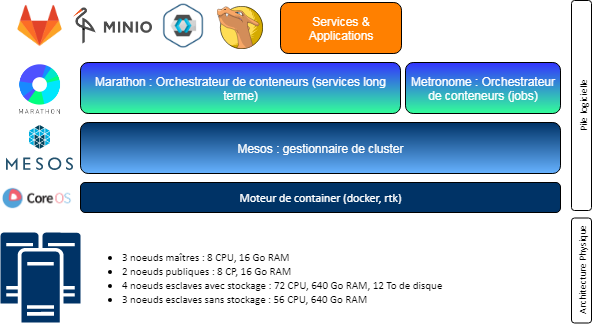
\includegraphics[scale=0.70]{images/Archi-inno.png}
  \caption{Architecture simplifiée de la plateforme Innovation}
  \label{fig:une-image}
\end{figure}
\vspace{10pt}

L'architecture physique totalise pour la gestion d'application 456 CPU, 4480 Go de RAM et 48 To de stockage disque. Côté logiciel, il s'agit d'un cluster \textbf{Mesos} utilisant \textbf{Marathon} et \textbf{Metronome} comme orchestrateur de conteneurs, accompagnés de plusieurs services longues durées (de gauche à droite sur le schéma):
\begin{enumerate}
    \item \href{https://about.gitlab.com/}{\textbf{Gitlab}} \cite{gitlab}~: la forge logicielle de la plateforme. Elle est dotée notamment d'un CI/CD (\textit{Continuous Integration / Continuous Delivery}), facilitant la mise à jour des services de la plateforme. La configuration des services de longue durée y est stockée~: chaque service longue durée a un projet Gitlab qui lui est associé, exception faite des services centraux (Gitlab, Minio). Les Gitlab-runners de la plateforme permettent, via Gitlab, de mettre à jour les services de la plateforme et d'en déployer de nouveaux en sollicitant l'API Marathon.
    \vspace{5pt}
    \item \href{https://min.io/}{\textbf{Minio}} \cite{minio}~: service de stockage réparti orienté objet. Minio est une implémentation de S3, \textit{Simple Storage System}, développé par \textbf{Amazon}. Il offre par conséquent une API compatible avec beaucoup de clients, en plus d'une interface Web pour gérer ses fichiers à la main.
    \vspace{5pt}
    \item \href{https://www.keycloak.org/}{\textbf{KeyCloak}} \cite{keycloak}~: service d'authentification et de gestion d'accès. Il fournit aux services une API pour gérer l'authentification. Il est notamment utilisé par Gitlab et par Minio (session).
    \vspace{5pt}
    \item \textbf{Onyxia}~: service web d'utilisation de la plateforme. Développé en interne, il regroupe une IHM et une API. L'IHM, portail d'entrée pour les utilisateurs de la plateforme, fournit la liste des services longues durées de la plateforme, une liste d'applications dites «~self~», que chacun peut lancer (des IDEs, outils bureautiques, etc.) ainsi qu'une IHM pour interagir avec Minio (déposer des fichiers par exemple). Afin de lancer un self-service, elle communique avec l'API REST Onyxia. Cette dernière dialogue avec Marathon et Mesos pour lancer le conteneur et ouvrir l'accès à l'utilisateur.
    \vspace{5pt}
    \item Et beaucoup d'autres applications ! \href{https://www.vaultproject.io/}{\textbf{Vault}} \cite{vault}, gestionnaire de secrets, \href{https://fr.sonatype.com/nexus-repository-sonatype}{\textbf{Nexus}} \cite{nexus}, gestionnaire de dépôt, \href{https://rocket.chat/}{\textbf{RocketChat}} \cite{rocketchat}, serveur de messagerie instantanée ou encore \href{https://humhub.org}{\textbf{Humhub}} \cite{humhub}, réseau social d'entreprise sont déployés sur Marathon.
    \newline
\end{enumerate}

La plateforme fournit également des services à la demande, ou self-services. La majorité d'entre eux est orientée développement ou statistique, mais certains sont des outils collaboratifs à la destination de tous. Elle totalise donc une soixantaine de services. Dans la continuité des missions de la DIIT, le but de la plateforme est également d'encourager le travail collaboratif, notamment autour de la gestion et l'entretien des services mis à disposition.

\subsubsection{Une approche collaborative}
Je découvre tout au long du stage un fonctionnement humain centré sur la collaboration et l'ouverture. Bien que celui-ci me soit familier de par mon engagement associatif à l'école, je l'observe à l'Insee sous une toute autre échelle et avec une diversité des profils. Certains services sont en effet maintenus aujourd'hui par des statisticiens, qui ont en général une vision pratique, une vision métier de l'informatique. Cela a été rendu possible par les incubations qu'offre la DIIT.
\newline

Ces incubations, auxquelles j'ai pu participer, durent deux ou trois jours. Elles ont pour but d'aider une équipe sur leur projet de développement. L'équipe vient avec une problématique technique relative aux méthodes de développement DevOps. Le but est de leur donner les outils et compétences pour être à même d'intégrer cette démarche~: elle inclut en général un apprentissage de \textbf{Git} lorsque cela est nécessaire, et plus souvent le fonctionnement de Gitlab-CI, de \textbf{Docker} et de Marathon. J'ai la chance lors de ces incubations d'en apprendre davantage sur la plateforme en explorant les différents cas d'usage, mais aussi en apportant mon aide aux incubés concernant l'utilisation de Git et de Docker par exemple. C'est ainsi que la DIIT favorise une gestion commune de la plateforme, les incubations aboutissant parfois au déploiement d'un nouveau service sur la plateforme, service géré principalement par l'équipe incubée. Suite à une incubation, deux statisticiens des bureaux de Marseille gèrent aujourd'hui un service \textit{OpenStreetMap} sur la plateforme, qui leur permet d'effectuer des statistiques sur les temps de trajet entre domicile et travail à partir des données du recensement.
\newline

Travaillant sur les environnements de développement disponibles en self-service, j'ai également contribué au projet \textbf{Desktop Ubuntu} de la plateforme. Ce service permet de développer simplement sous un Ubuntu web, notamment en Java. Pour plus de confort et d'efficacité dans le développement, je contribue à l'image Docker Ubuntu proposé, en mettant à jour les IDEs et en y ajoutant certains plugins et paquets.
\label{section 2.2.2}

\subsubsection*{Le séminaire du développement}
Les échanges sur les nouveaux projets et technologies utilisées sont favorisés par un évènement qui a lieu chaque année et auquel j'ai eu la chance de participer~: le séminaire du développement. Pendant une semaine, chaque équipe de développement de l'Insee, incluant des équipes à Nantes, Lille et Orléans, a l'occasion de présenter à tous les développeurs les utilisations de nouvelles technologies dans leurs travaux.
\newline

Ce séminaire a été l'occasion pour moi de voir beaucoup de technologies et bibliothèques récentes en application concrète dans des projets. Écriture de grammaire avec \textbf{Antlr4}, automatisation de tests d'interface Web avec \textbf{Selenium} et \textbf{Cypress}, ou encore packaging d'applications Python pour du web avec \textbf{Flask}, le séminaire offre une bonne vue d'ensemble des technologies à l'oeuvre à l'Insee. J'ai moi aussi eu l'occasion de présenter mes premiers résultats sur l'utilisation du traitement du langage naturel dans les publications de l'institut. Des échanges sur les différentes bibliothèques existantes me permettent de mettre à l'épreuve le premier pipeline construit, et ainsi de l'améliorer.
\newline

La démarche participative de la plateforme est favorisée jusque dans les salles serveurs ! Avec l'arrivée de quatre nouvelles machines, j'ai apporté mon aide pour remplacer les noeuds esclaves de stockage de la plateforme innovation. Au programme~: câblage, configuration réseau et installation de système d'exploitation. 

\begin{figure}[H]
    \centering
    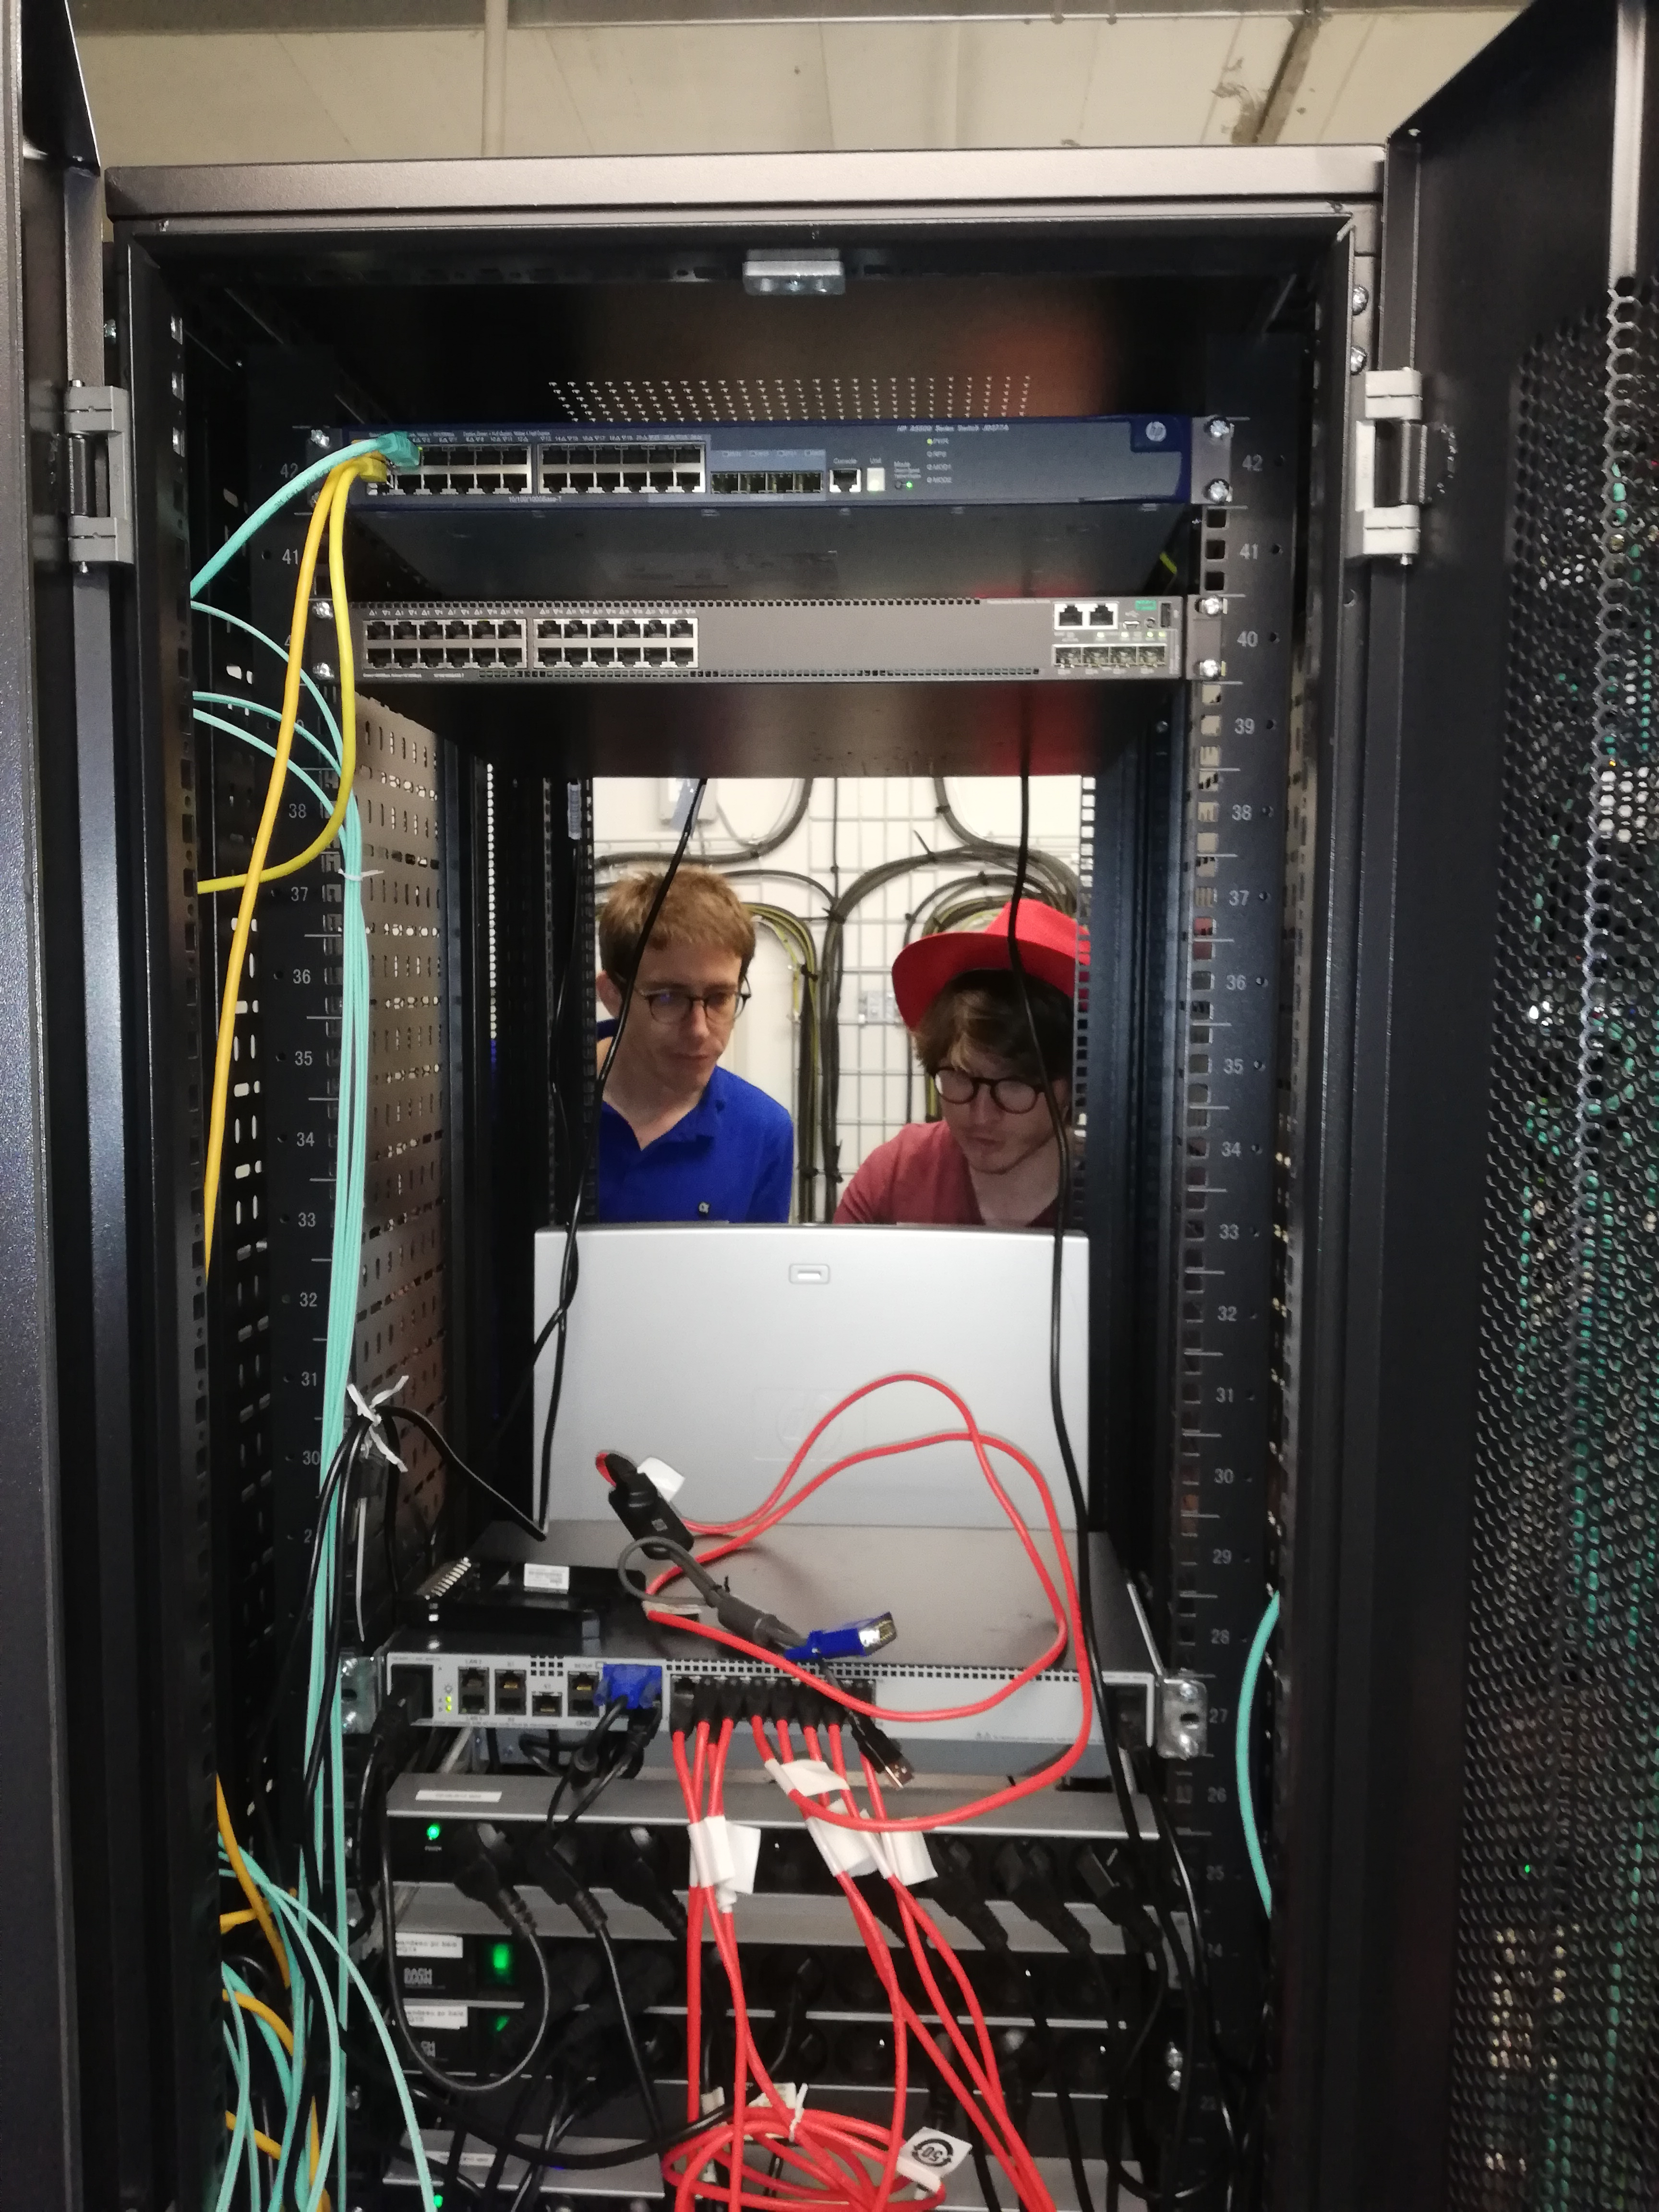
\includegraphics[scale=0.10]{images/salle-machine.jpg}
    \caption{Frédéric Comte (à gauche) et moi-même (à droite) en salle machine}
    \label{fig:salle-machine}
\end{figure}
\vspace{10pt}

C'est dans cette démarche collaborative autour du développement que j'ai d'une part adopté la pratique DevOps et d'autre part aidé des agents Insee autour de cette pratique.
\label{section 2.2.2 - Séminaire du développement}

\subsubsection{La pratique DevOps}
La pratique DevOps est le fait de développer un projet de manière continue, du développement du logiciel cœur jusqu'à sa livraison et sa maintenance pour l'utilisateur final. Souvent accompagné d'une démarche agile, il s'agit dans cette méthode d'assurer et de suivre toutes les étapes de vie d'un logiciel~: développer, intégrer, tester, déployer, exploiter et maintenir les fonctionnalités d'une application de manière continue. Le principe est de faire des cycles de développement courts, et des livraisons fréquentes, afin de mieux s'adapter aux changements. L'automatisation de certaines tâches, comme le déploiement ou les tests, fait pleinement partie de cette démarche.
\newline

La plateforme, avec \textbf{GitLab-CI/CD}, \textbf{Nexus} et l'API \textbf{Onyxia}, offre tous les outils pour adopter la démarche. Pour mon premier pipeline réalisé en Java et utilisant le gestionnaire de dépendances \textbf{Maven}, j'ai pu mettre en place un pipeline GitLab qui teste mon application dans un environnement proche d'un environnement de production. C'est en effet l'un des avantages du DevOps~: préparer le terrain le plus en amont possible pour un passage en production. Le but n'est pas que de déployer une application fonctionnelle, mais de détecter les points d'amélioration sur le code existant. 
\newline

Pour la première maquette de mon application, il s'agit simplement de créer un pipeline GitLab permettant d'exécuter du code Java. Concrètement, cela se présente sous la forme d'un fichier, \textit{.gitlab-ci.yml}, qui spécifie les étapes de mon pipeline. Chaque étape correspond au déploiement d'un conteneur Docker sur la plateforme, dont l'image utilisée est spécifiée dans le fichier. Dans notre cas, l'image utilisée inclue le JDK-8 (Java 8) ainsi que le gestionnaire de dépendances Maven. Il suffit ensuite d'indiquer les lignes de commande shell à exécuter pour effectuer les tests. Pour un projet fait avec \textbf{Maven}, les commandes à exécuter sont simples. La récupération des données l'est moins~: en effet, Gitlab ne publie par défaut que la sortie standard et la sortie d'erreur du conteneur. Dans le cas d'un déploiement, il est parfois nécessaire de conserver des fichiers écrits par l'application dans le conteneur. Nous y reviendrons dans la partie \ref{section 3.2.3} pour la description de la deuxième version du service.
\label{section 2.2.3}

\subsubsection{Les différentes méthodes testées}
Les premiers tests sur les méthodes de REN à base de règles ont été réalisés avec la bibliothèque \href{https://stanfordnlp.github.io/CoreNLP/}{Stanford Core NLP} \cite{corenlp-doc}. Ce choix a été guidé par l'orientation recherche de la bibliothèque~: l'intégration des dernières avancées techniques dans le TLN est préférée à la stabilité. C'est en effet parmi les premières à proposer en 2015 des traitements basés sur le \textit{Deep Learning}. Écrite en Java, elle me permet en plus de concentrer mes efforts sur la méthode de REN et non sur l'implémentation. 
\newline

J'ai d'abord travaillé sur la reconnaissance des concepts statistiques à partir de leur libellé. Ces derniers ont diverses formes, avec parfois des annotations qu'on ne retrouve pas dans les publications. J'ai donc éliminé pour les tests les concepts dont les libellés ont des parenthèses et les longs libellés avec énumération, ce qui laisse environ 700 concepts. Une difficulté majeure pour tester les méthodes de reconnaissance est l'obtention de données de tests fiables et représentatives~: d'une part, bien que la majorité des mentions de concepts statistiques soit aisée à repérer, certains utilisant des mots très communs ne le sont pas pour des non-spécialistes. D'autre part, les publications traitent généralement d'un sujet précis. Une publication ne sollicite finalement que peu de concepts statistiques, une dizaine en général. Il est donc difficile d'estimer la pertinence d'une méthode et c'est pourquoi je me suis attaché dans ces tests à reconnaître les groupes de mots pouvant être une occurrence de concept statistique. Les deux publications utilisées pour les tests sont tirées de la même collection~: \href{https://insee.fr/fr/statistiques/4129807}{Insee Première 1750} et \href{https://insee.fr/fr/statistiques/3703745}{Insee Première 1734}.
\newline

La toute première méthode testée est la plus triviale~: reconnaître les occurrences en faisant une simple recherche textuelle. Cette simple méthode permet déjà de trouver beaucoup d'occurrences de concepts, souvent ceux ayant des libellés courts et simples, comme «~salaire~» ou «~commune~». Pour identifier les autres occurrences, plusieurs outils de TLN peuvent être utilisés~:
\newline

\begin{itemize}
    \item \textit{Lemmatization}~: c'est le premier traitement à tester. La méthode utilisant la lemmatisation consiste à créer des règles indiquant des suites de lemmes, par exemple~: «~Toutes les suites de quatre tokens consécutifs ayant respectivement pour lemme \textit{petit}, \textit{et}, \textit{moyen}, et \textit{entreprise}~». Cela permet de s'affranchir du contexte grammatical~: qu'il soit cité au singulier comme dans le libellé, ou au pluriel, qui est la forme la plus couramment utilisée dans les publications, la règle utilisant les lemmes permet d'étiqueter le concept. Il est difficile d'effectuer le test avec Core NLP, la bibliothèque ne fournissant pas de lemmatisation pour le français. La bibliothèque fournit une interface permettant de créer son propre lemmatiseur. À l'aide d'un dictionnaire de lemmes, mis en ligne par \textit{Europeana} et disponible sur \href{http://www.iramuteq.org/}{Iramuteq} \cite{iramuteq}, j'ai construit mon propre lemmatiseur. Le principe est simplement d'associer à chaque mot son lemme. Sur les deux publications testées, l'implémentation de la méthode a permis de repérer plus de 120 occurrences dans chaque texte.
    \newline
    
    \item \textit{Part-of-Speech}~: l'idée derrière l'utilisation de ce traitement est d'améliorer la méthode décrite précédemment. La quasi-totalité des mentions de concepts dans les publications sont des groupes nominaux. Le nom principal est généralement présent mais les qualificatifs ne correspondent pas toujours à ceux utilisés dans les libellés~: il y en a parfois davantage, modifiant le libellé, parfois moins, les autres qualificatifs étant sous-entendus et dépendant souvent du contexte. «~salaire net moyen en EQTP~» fait par exemple référence à «~salaire en équivalent temps plein~». L'idée est donc de construire des règles comme celle-ci~: «~Tous les groupes nominaux dont le nom principal a pour lemme \textit{entreprise} dont au moins deux adjectifs ont pour lemmes \textit{petit} et \textit{moyen}~». Les tests sont plutôt concluants~: 177 concepts sont repérés dans la première publication et 181 dans la seconde.
    \newline
\end{itemize}

Les premiers tests sont encourageants mais ne couvrent qu'une petite partie des concepts de la base. Les règles sont de plus écrites à la main pour les quelques concepts testés. Pour passer à une plus grande échelle, j'ai construit un premier service de REN, incluant un générateur de règles.
\label{section 2.2.4}

\subsubsection{Premier service de REN}
Le premier service de reconnaissance d'entités nommées est construit avec la bibliothèque Stanford Core NLP. Afin qu'il soit modifiable et puisse aisément s'intégrer dans un pipeline GitLab-CI, l'architecture suivante est adoptée~:

\begin{figure}[H]
    \centering
    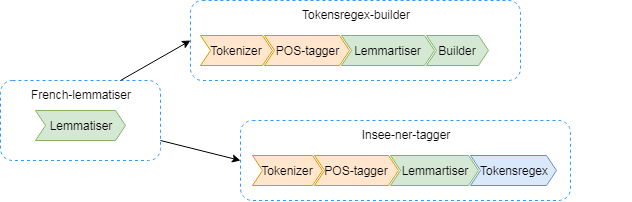
\includegraphics[scale=0.38]{images/Concept-tagger.png}
    \caption{Schéma fonctionnel du premier service de REN}
    \label{fig:premier-pipeline}
\end{figure}
\vspace{10pt}

L'architecture du service se décompose en trois modules~: 
\begin{itemize}
    \item \textit{French-lemmatiser}~: un module contenant la classe \textit{French-lemmatiser} et le dictionnaire de lemmes. C'est le composant associant à chaque token un lemme. La séparation du lemmatiseur en un seul module est un choix guidé par une exigence d'adaptabilité du code. La méthode de génération de règles doit être valable pour plusieurs langues, et le lemmatiseur est un composant spécifique à la langue. C'est pourquoi séparer ce composant en en faisant un module permet de passer facilement d'une langue à une autre.
    \vspace{5pt}
    \item \textit{Tokensregex-builder}~: il s'agit du générateur de règles, appelé «~ Tokensregex~» dans la bibliothèque Stanford Core NLP. Il prend en entrée une liste de groupes nominaux représentant des entités nommées et génère un fichier de règles au format spécifié par la bibliothèque. Elles sont générées en faisant tourner un pipeline Stanford Core NLP ayant les quatre composants décrits ci-dessus. Le composant \textit{Builder} prend en entrée les libellés annotés et donne en sortie des règles suivant ce schéma~: 
    \vspace{10pt}
    \begin{figure}[H]
        \centering
        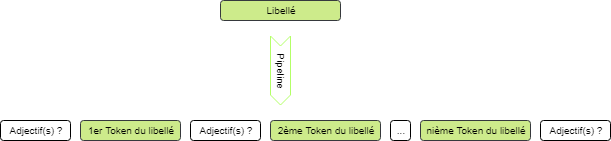
\includegraphics[scale=0.6]{images/Exemple-tokensregex.png}
        \caption{Schéma du construction d'une \textit{Tokensregex}}
        \label{fig:schema-tokensregex}
    \end{figure}
    \vspace{10pt}
    La sous-règle «~[1er, 2e, ...n]ième Token du libellé~» repère un token ayant le même lemme et la même nature grammaticale que le token du libellé. Cette fonctionnalité a été séparée en un module dans une volonté de produire du code réutilisable. Il n'est d'une part pas spécifique à l'Insee, et d'autre part il pourrait s'appliquer à d'autres langues.
    \vspace{5pt}
    \item \textit{Insee-ner-tagger}~: le module spécifique à l'Insee qui intègre le pipeline qui va traiter le texte des publications. Il contient deux classes~: la première est le pipeline Stanford Core NLP configuré pour reconnaître les concepts statistiques. Le fichier de sortie de \textit{Tokensregex-builder}, fichier de règles, figure parmi les ressources et est lu par le composant \textit{Tokensregex} qui annote le texte en fonction. La seconde classe gère le format XML des publications. Elle consiste en un processeur XSLT (langage de manipulation de fichiers XML), et en une feuille de style XSLT appelant le pipeline sur le contenu des balises désirées.
    \newline
\end{itemize}

Les interfaces sont conçues dans un souci de testabilité~: un autre module de test vient compléter cette liste. Ce dernier assure simplement la communication avec les différentes bases de données pour obtenir les publications souhaitées et ainsi tester le pipeline. Un client PostgreSQL permet d'obtenir les métadonnées sur les publications (leur type, la langue d'écriture, leurs identifiants, etc.), et permet d'obtenir les identifiants des publications que l'on peut obtenir via un serveur HTTP. Ces deux clients nous donnent les publications au format XML, et le programme principal le même fichier enrichi de balises XML repérant les occurrences de concepts. Pour plus de lisibilité lors de la vérification des concepts matchés, le module de texte inclut une seconde transformation XSLT afin d'obtenir un rendu HTML.
\newline

Mon pipeline de test se présente comme suit~:
\vspace{10pt}
\begin{figure}[H]
    \centering
    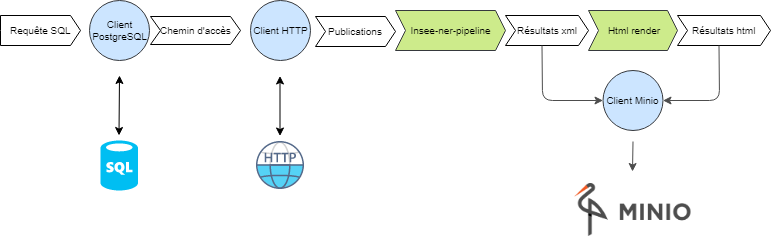
\includegraphics[scale=0.56]{images/Pipeline-test.png}
    \caption{Schéma du pipeline de test du service}
    \label{fig:pipeline-test}
\end{figure}
\vspace{10pt}

Il est lancé à chaque mise à jour du dépôt Git central, sur n'importe quelle branche, et enregistre les résultats sous format XML et HTML dans Minio.
\newline

\subsubsection*{Résultats à grande échelle}
Le pipeline est testé sur les publications \textit{Insee Première}, collection rassemblant des publications riches en données textuelles. Une rapide analyse statistique sur la couverture des concepts mentionnés ainsi que sur leur fréquence d'apparition révèle certaines lacunes du pipeline. Trois sont décrites ci-dessous.
\newline

Premièrement, la lemmatisation est lacunaire~: en effet, la connaissance seule de l'orthographe d'un mot ne suffit pas à donner le mot du dictionnaire associé. Par exemple, le mot «~moyen~» peut correspondre à l'adjectif ou bien au nom. C'est pour cela que le concept «~petite et moyenne entreprise~» n'est jamais reconnu~: «~moyenne~» est lemmatisée en le nom «~moyenne~», désignant la moyenne statistique, tandis que le mot «~moyennes~» est lemmatisé en l'adjectif «~moyen~» dans le dictionnaire de lemmes utilisés. Ce dernier n'est d'ailleurs pas complet et ne propose pas de lemme pour certains mots peu fréquents tels que «~multipolarisé~». Une solution est de ne pas utiliser seulement l'orthographe du mot pour trouver son lemme, mais également sa nature grammaticale. Cette solution n'est pas simple à mettre en oeuvre. Il s'agit de trouver ou générer un dictionnaire < < mot, nature >, lemme >.
\newline

Deuxièmement, la tokenization est destructive~: cette étape permet de découper le texte en mots et éléments de ponctuation. Dans la plupart des cas cela est simple. Les quelques exceptions sont les contractions de certains mots, comme «~de~» et «~le~» contracté en «~du~». La correction est toutefois réalisable en répertoriant les cas de contraction et en ajoutant un composant reconstruisant ces mots en fin de traitement.
\newline

Troisièmement, les règles générées n'affichent parfois pas la bonne nature grammaticale des mots des libellés. Le \textit{Part-of-Speech tagging} utilise, pour déterminer la nature grammaticale d'un mot, tous les éléments de la phrase dans laquelle on le trouve. Cela explique les erreurs commises lorsque l'on ne soumet qu'un groupe nominal. En ajoutant une phrase donnant les éléments de contexte autour du concept avant de l'analyser, cela diminue fortement les erreurs.
\newline

Intégration des libellés alternatifs (voir section \ref{section 1.2.1}), reconnaissance de concepts géographiques, de dates, et correction du lemmatiseur~: globalement, le pipeline est largement améliorable à l'heure actuelle. Mais le but est davantage ici d'explorer les possibilités de Stanford Core NLP directement sur les publications, et non de créer un service pérenne. De plus, des mises à jour récentes sur l'autre bibliothèque de TLN largement utilisée, \textbf{SpaCy}, posent la question du choix de bibliothèque.
\label{section 2.2.5}

\subsection*{Conclusion}
La mise en oeuvre de ce premier pipeline, facilitée à la fois par les outils de la plateforme et par la possibilité de les adapter aux besoins, m'a beaucoup apporté sur les problématiques de la REN dans le contexte Insee. Cela nourrit une réflexion plus approfondie et plus mûre sur le sujet, et rend possible la valorisation de mes acquis d'architecte de services informatiques répartis.
